\chapter{Introduction} \label{sec:introduction}

The Roa Logic AHB-Lite APB4 Bridge is a fully parameterized soft IP
interconnect bridge between the \emph{AMBA 3 AHB-Lite v1.0} and
\emph{AMBA APB v2.0} bus protocols.

The AHB-Lite APB4 Bridge natively supports a \emph{single} peripheral,
however \emph{multiple} APB4 peripherals may be connected to a single
bridge by including supporting multiplexer logic -- See the \emph{AMBA
APB v2.0 Protocol} specification. An \emph{APB4 Multiplexer} IP
implementing this capability is available from Roa Logic

\begin{figure}[tbh]
	\centering
	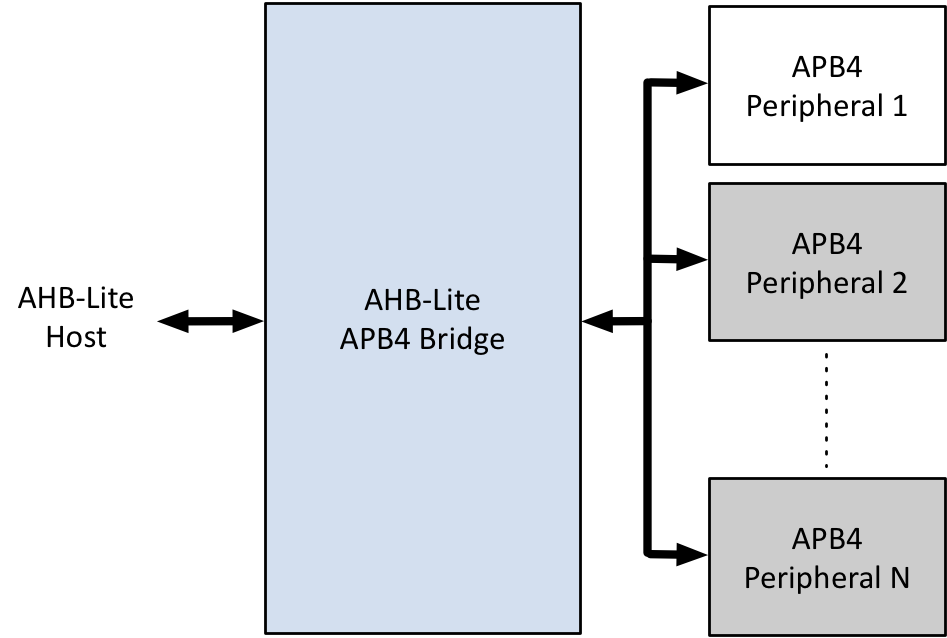
\includegraphics{assets/img/apb4-bridge-per.png}
	\caption{APB4 Bridge with Multiple Peripherals}
	\label{fig:apb4-bridge-sys}
\end{figure}


\section{Features}\label{sec:features}

\begin{itemize}
  \item
    Full support for AMBA 3 AHB-Lite and APB version 2.0 (APB4) protocol
  \item
    Fully parameterized
  \item
    Unlimited APB4 address and data widths supported
  \item
    Configurable number of peripheral-side byte lanes with automatic
    handling of burst transfers
  \item
    Support for separate clock domain per interface with automatic
    handling of cross-domain timing.
\end{itemize}